\documentclass[a4paper,10pt,oneside]{article}
\usepackage[polutonikogreek,italian]{babel}
\usepackage[utf8x]{inputenc}
\usepackage{amsmath}
\usepackage{amsthm}
\usepackage{amssymb}
\usepackage{amscd}
\usepackage{graphicx}
\usepackage{float}
\usepackage{array}
\usepackage{rotating}
\usepackage[small]{caption}
\usepackage{lscape}
\usepackage{fancybox}
\usepackage{booktabs}
\usepackage[noanswer]{exercise}
\parindent0ex
\renewcommand{\fboxsep}{0.4cm}
\usepackage{hyperref}
\renewcommand{\textfraction}{0.05}
\renewcommand{\topfraction}{0.95}
\renewcommand{\bottomfraction}{0.95}
\renewcommand{\floatpagefraction}{0.35}
\renewcommand{\ExerciseName}{Esercizio}
\renewcommand{\ExerciseListName}{Es}
\setcounter{totalnumber}{5}
\restylefloat{figure}
\begin{document}
\thispagestyle{empty}
 \section*{Moto circolare uniforme}
\vspace{1cm}

In fisica il \emph{moto circolare} consiste nel moto di un punto materiale lungo una circonferenza, parleremo di \emph{moto circolare uniforme} quando il modulo della velocità del punto materiale lungo la circonferenza è costante. Per studiare quest'ultimo caso particolare  introduciamo alcune grandezze che saranno di grande utilità nella definizione dei vettori \textbf{posizione}, \textbf{velocità} e \textbf{accelerazione}. La prima delle nuove grandezze che andremo ad utilizzare prende il nome di \emph{periodo}. Il periodo è definito come l'intervallo di tempo necessario affinché il punto materiale ripassi per lo stesso punto della circonferenza o in altre parole il tempo necessario per compiere un ciclo. Di seguito indicheremo il periodo con la lettera $T$ chiaramente l'unità di misura del periodo è il secondo. La seconda grandezza che sarà necessaria per la trattazione del moto circolare è la \emph{velocità angolare}\footnote{Nella nostra trattazione semplificata la velocità angolare è uno scalare e non un vettore} che nel caso del moto circolare uniforme può essere definita come:
\begin{equation}\label{eq:vel_ang}
 \omega=\frac{2\pi}{T}
\end{equation}
come si evince dalla [\ref{eq:vel_ang}] la velocità angolare rappresenta il numero di radianti spazzati in un secondo dal vettore che congiunge il punto materiale al centro della circonferenza. La velocità angolare si misura in $s^{-1}$ ovvero ha le dimensioni del reciproco di un tempo. Ad esempio se un oggetto ha una velocità angolare $\omega=2\pi\ s^{-1}$ significa che in un secondo il punto materiale ha compiuto un intero giro (dato che l'angolo giro misura $2\pi$ radianti). Da ultima introduciamo la \emph{frequenza} ovvero il numero di volte che un dato fenomeno si ripete nell'unità di tempo. Definiamo la frequenza come:
\begin{equation}\label{eq:freq}
 \nu=\frac{1}{T}
\end{equation}
vediamo che la frequenza è il reciproco del periodo ad esempio se un dato fenomeno ha un periodo di $0.5s$ la sua frequenza sarà $2Hz$. Ricordiamo che l'unità di misura della frequenza è l'Hertz (Hz).

\subsection*{Il vettore posizione}

Per definire il vettore posizione facciamo riferimento alla figura [\ref{fig:vet_posizione}]. Vediamo che l'angolo che il vettore posizione forma con l'asse delle ascisse al tempo $t$ è $\omega t$ (questo angolo è variabile ed aumenta all'aumentare di $t$), possiamo quindi calcolare, utilizzando le note relazione trigonometriche, le proiezioni del vettore posizione $\mathbf{r}$ sugli assi coordinati ottenendo:
\begin{equation}
 r_x=r\cos(\omega t)
\end{equation}
dove $r=|\mathbf{r}|$ e la proiezione sull'asse delle ordinate:
\begin{equation}
 r_y=r\sin(\omega t)
\end{equation}


\begin{figure}[H]
\begin{center}
 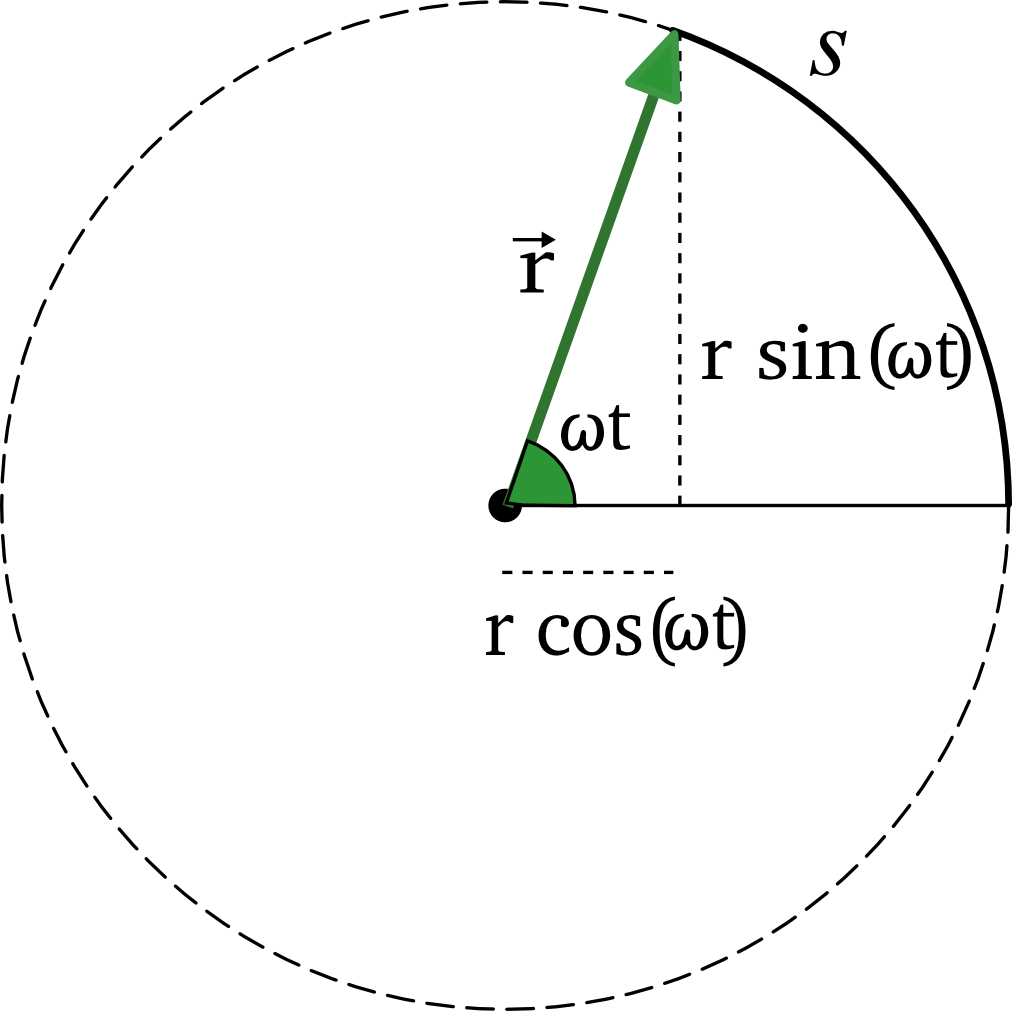
\includegraphics[width=0.4\textwidth]{./immagini/vet_posizione.png}
 % vet_posizione.png: 1012x1137 pixel, 303dpi, 8.48x9.53 cm, bb=
 \caption{Il vettore posizione nel moto circolare uniforme}
 \label{fig:vet_posizione}
\end{center}
\end{figure}

unendo i due risultati precedenti possiamo ricavare il vettore posizione del punto materiale che si muove di moto circolare uniforme:
\begin{equation}
 \mathbf{r}=\left(r\cos(\omega t),r\sin(\omega t)\right)
\end{equation}
\subsection*{Il vettore velocità}
Sappiamo per ipotesi (dato che intendiamo trattare unicamente moti circolari uniformi) che il modulo della velocità della particella lungo la circonferenza è costante quindi $|\mathbf{v}|=k$. Possiamo quindi calcolare il modulo della velocità basandoci sul raggio della circonferenza e sul periodo del punto materiale. Dalla conoscenza del raggio possiamo dedurre la lunghezza della circonferenza $c=2\pi r$ siccome tale lunghezza viene percorsa con velocità in modulo costante in un tempo pari a un periodo $T$ applicando le leggi della cinematica unidimensionale \footnote{Immaginiamo di srotolare la circonferenza e di percorrere a velocità costante un tratto rettilineo di lunghezza $c$} possiamo scrivere:
\begin{equation}
 v=|\mathbf{v}|=\frac{2\pi r}{T}
\end{equation}
o ricordando la definizione di velocità angolare:
\begin{equation}
 v=\omega r
\end{equation}
Per calcolare le componenti del vettore velocità senza fare ricorso a della matematica troppo complessa facciamo riferimento alla figura [\ref{fig:vet_veloc}].
\begin{figure}[H]
\begin{center}
 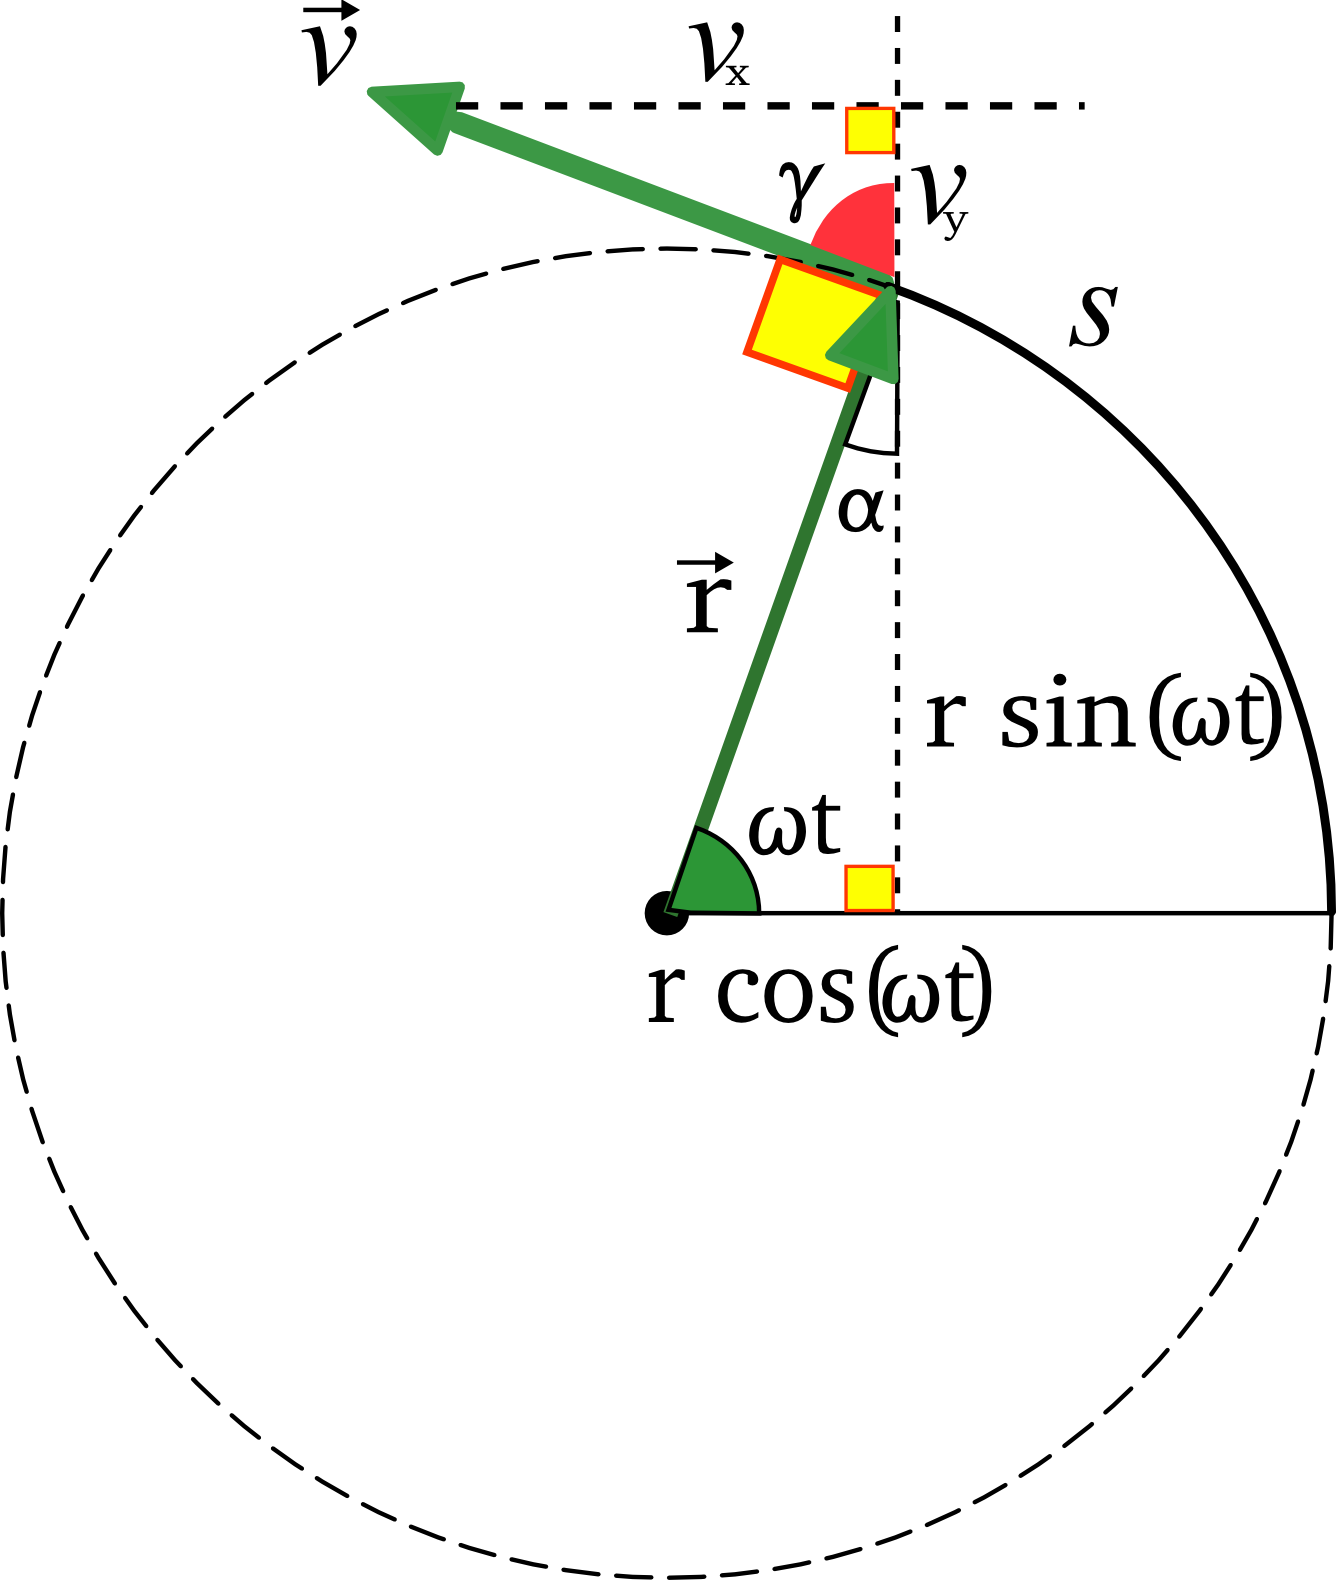
\includegraphics[width=0.4\textwidth]{./immagini/vet_velocita.png}
 % vet_velocita.png: 1430x1692 pixel, 428dpi, 8.48x10.03 cm, bb=
 \caption{Il vettore velocità di particella che si muove di moto circolare uniforme, il verso di rotazione è antiorario}
 \label{fig:vet_veloc}
\end{center}
\end{figure}
Dalla figura [\ref{fig:vet_veloc}] possiamo dedurre che l'angolo $\gamma$ misura $\omega t$ radianti dato che l'angolo che ha tale ampiezza e $\gamma$ sono entrambi complementari ad $\alpha$ questo ci permette di calcolare, utilizzando la trigonometria, le componenti $v_x$ e $v_y$ della velocità all'istante $t$:
\begin{equation}\label{eq:vx}
 v_x=-v\sin(\omega t)=-\omega r \sin(\omega t)
\end{equation}
dove nella [\ref{eq:vy}] il segno meno è dovuto al fatto che la componente $x$ della velocità ha verso opposto alla componente $x$ del vettore posizione e
\begin{equation}\label{eq:vy}
 v_y=v\cos(\omega t)=\omega r\cos (\omega t)
\end{equation}
nelle due equazioni precedenti notiamo come seno e coseno si siano scambiati rispetto al vettore posizione, combinando la  [\ref{eq:vy}] e la [\ref{eq:vx}] possiamo scrivere il vettore velocità:
\begin{equation}
 \mathbf{v}=\left(-\omega r \sin (\omega t),\omega r \cos (\omega t)\right)
\end{equation}

\subsection*{Il vettore accelerazione}

Ricordiamo che il vettore accelerazione media è definito come:
\begin{equation}\label{eq:acc_media}
 \mathbf{a}_m=\frac{\Delta \mathbf{v}}{\Delta t}
\end{equation}
nel moto circolare uniforme, benché il modulo della velocità sia costante, esiste una accelerazione che è responsabile della variazione di direzione e verso del \emph{vettore} velocità. Per determinare il  vettore accelerazione  media cerchiamo, per prima cosa, di calcolarne direzione e verso, dal risultato ottenuto  estrapoleremo poi il vettore accelerazione istantanea.
Dall'equazione [\ref{eq:acc_media}] notiamo come il vettore accelerazione media avrà lo stesso verso e la stessa direzione del vettore variazione di velocità $\Delta \mathbf v$. In figura [\ref{fig:accel1}] è stato disegnato il vettore variazione di velocità tra la posizione $\mathbf{r}_1$ e la posizione $\mathbf{r}_2$, possiamo notare che al diminuire  della lunghezza dell'arco $S$ il vettore $\mathbf{v}_2 -\mathbf{v}_1$ tende a disporsi lungo un raggio della circonferenza come in figura [\ref{fig:acce2}].
\begin{figure}[H]
\begin{center}
 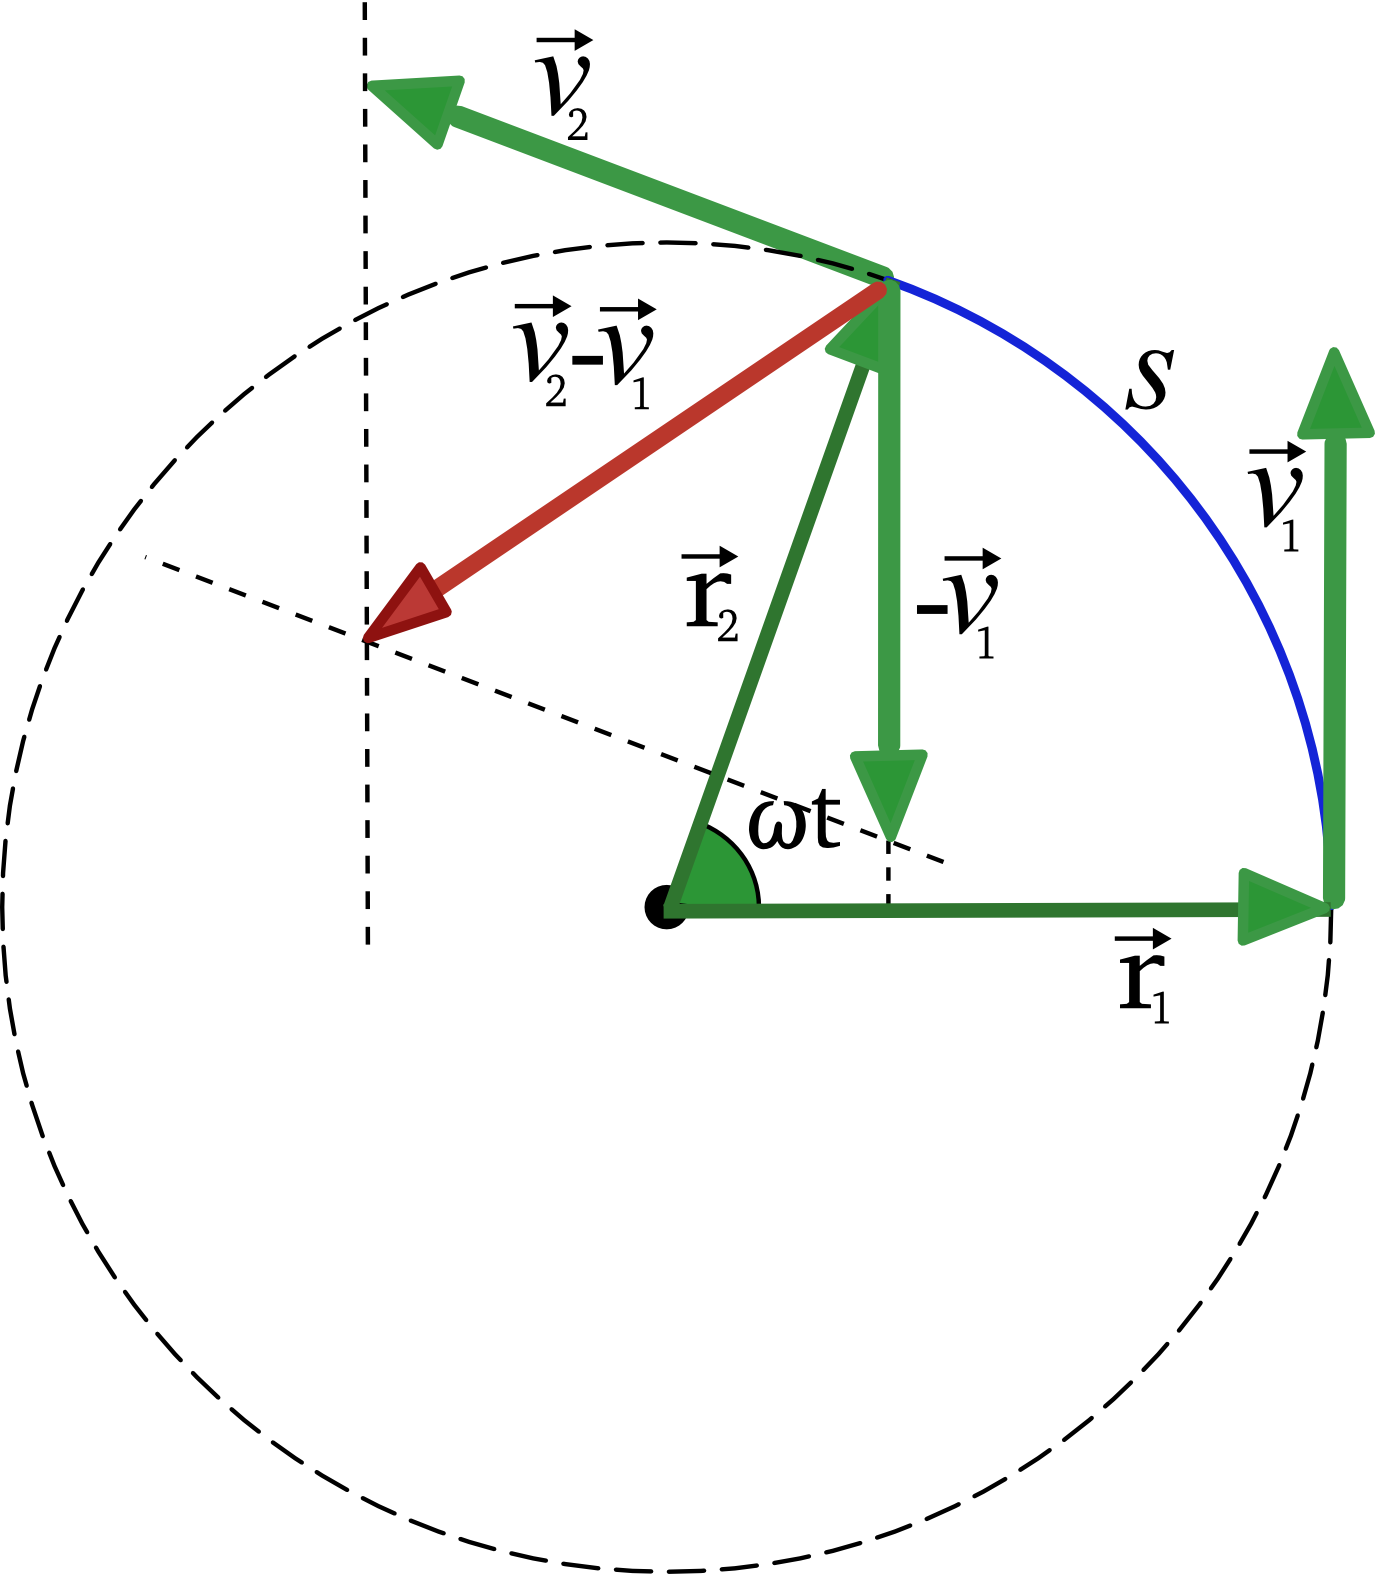
\includegraphics[width=0.4\textwidth]{./immagini/vet_acce.png}
 % vet_acce.png: 1375x1574 pixel, 400dpi, 8.73x9.99 cm, bb=0 0 248 283
 \caption{Il vettore accelerazione media punto verso l'interno, il vettore accelerazione istantanea ha la stessa direzione del vettore posizione ma verso opposto}
 \label{fig:accel1}
\end{center}
\end{figure}
\begin{figure}[H]
 \centering
 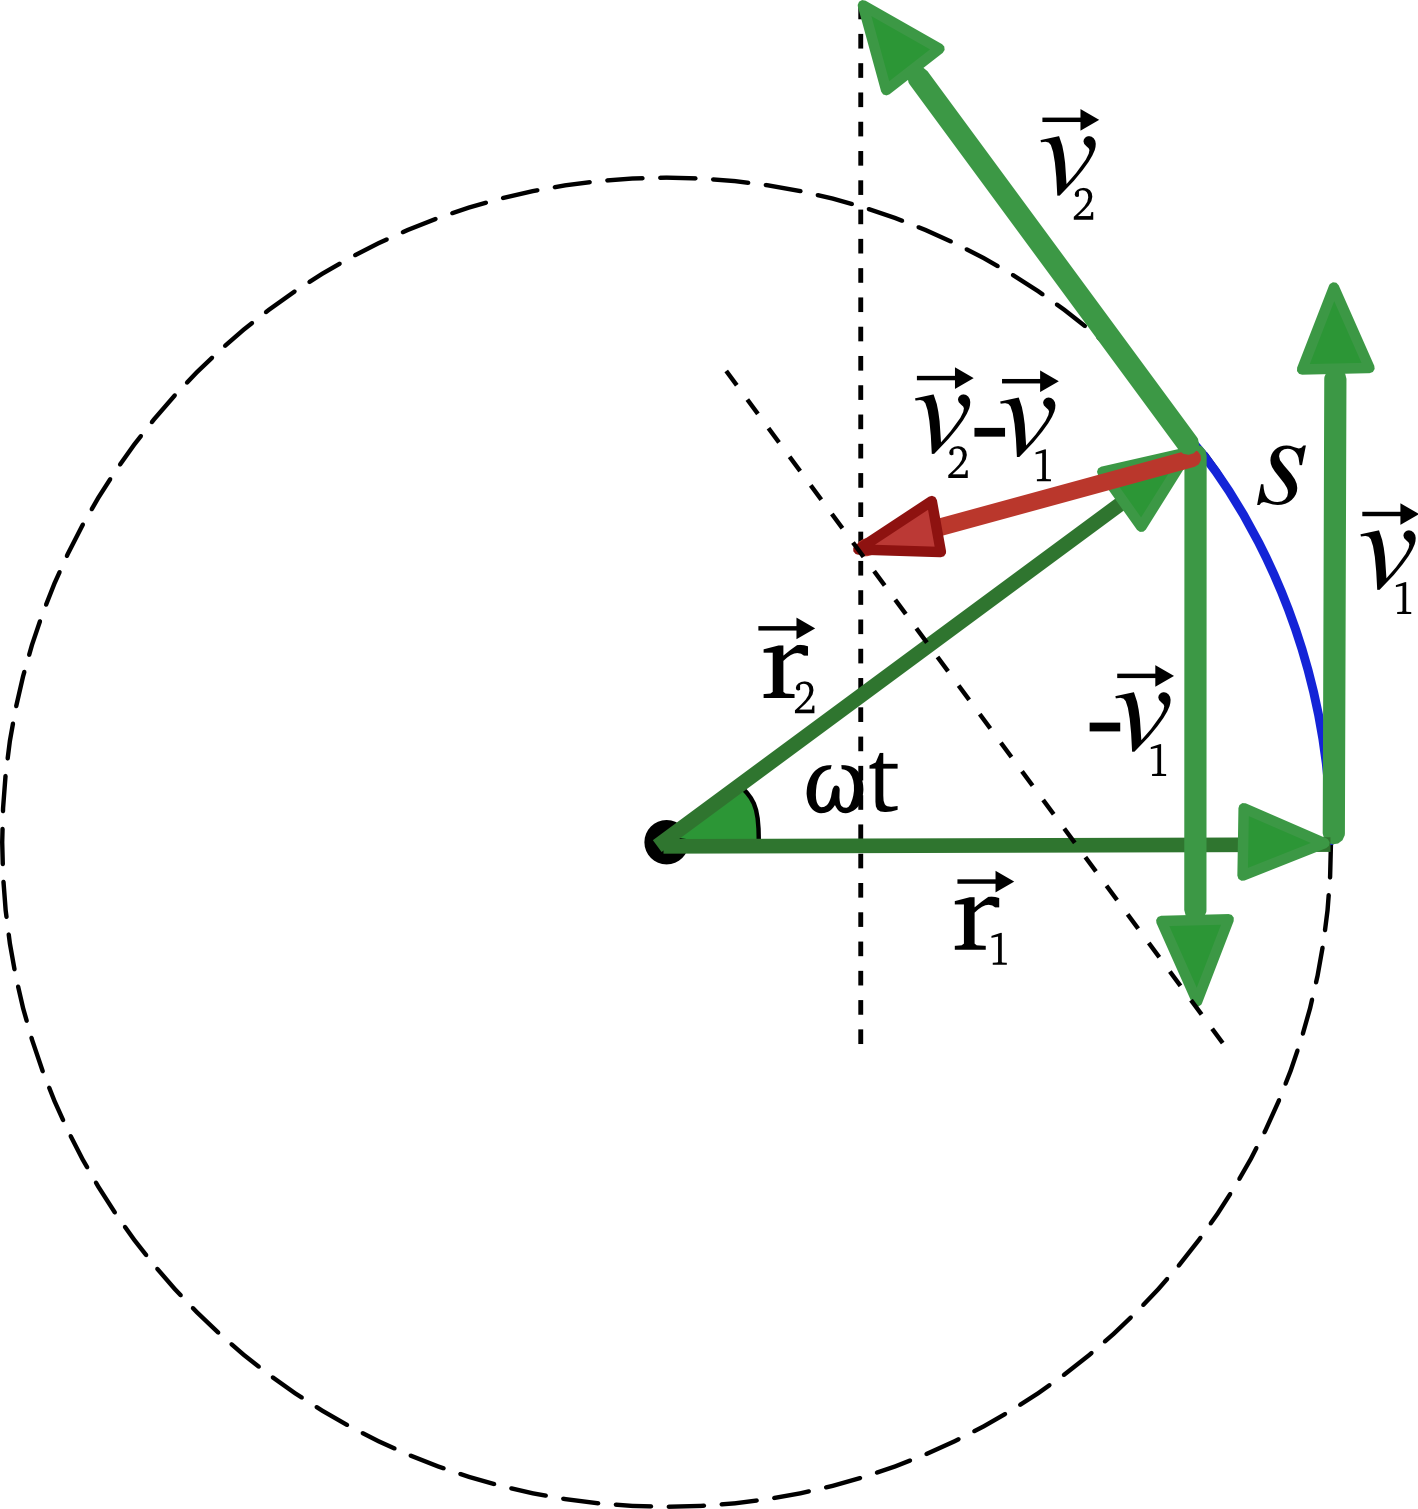
\includegraphics[width=0.4\textwidth]{./immagini/vet_acce2.png}
 % vet_acce2.png: 1418x1509 pixel, 400dpi, 9.00x9.58 cm, bb=
 \caption{Al diminuire della lunghezza dell'arco $S$ la direzione del vettore variazione di velocità tende alla direzione del vettore $\mathbf{r}_2$}
 \label{fig:acce2}
\end{figure}
Da quanto detto, risulta evidente che se consideriamo degli intervalli temporali $\Delta t$ molto piccoli rispetto al periodo $T$ possiamo scrivere il vettore accelerazione istantanea come:
\begin{equation}
 \mathbf{a}=\left(-a\cos(\omega t),-a\sin(\omega t)\right)
\end{equation}
dove i segno meno sono dovuti al verso opposto del vettore $\mathbf{a}$ rispetto al vettore $\mathbf{r}$ e $a$ rappresenta il modulo del vettore accelerazione. Per calcolare $a$ seguiamo lo schema di figura [\ref{fig:cal_acc}].
\begin{figure}[H]
 \centering
 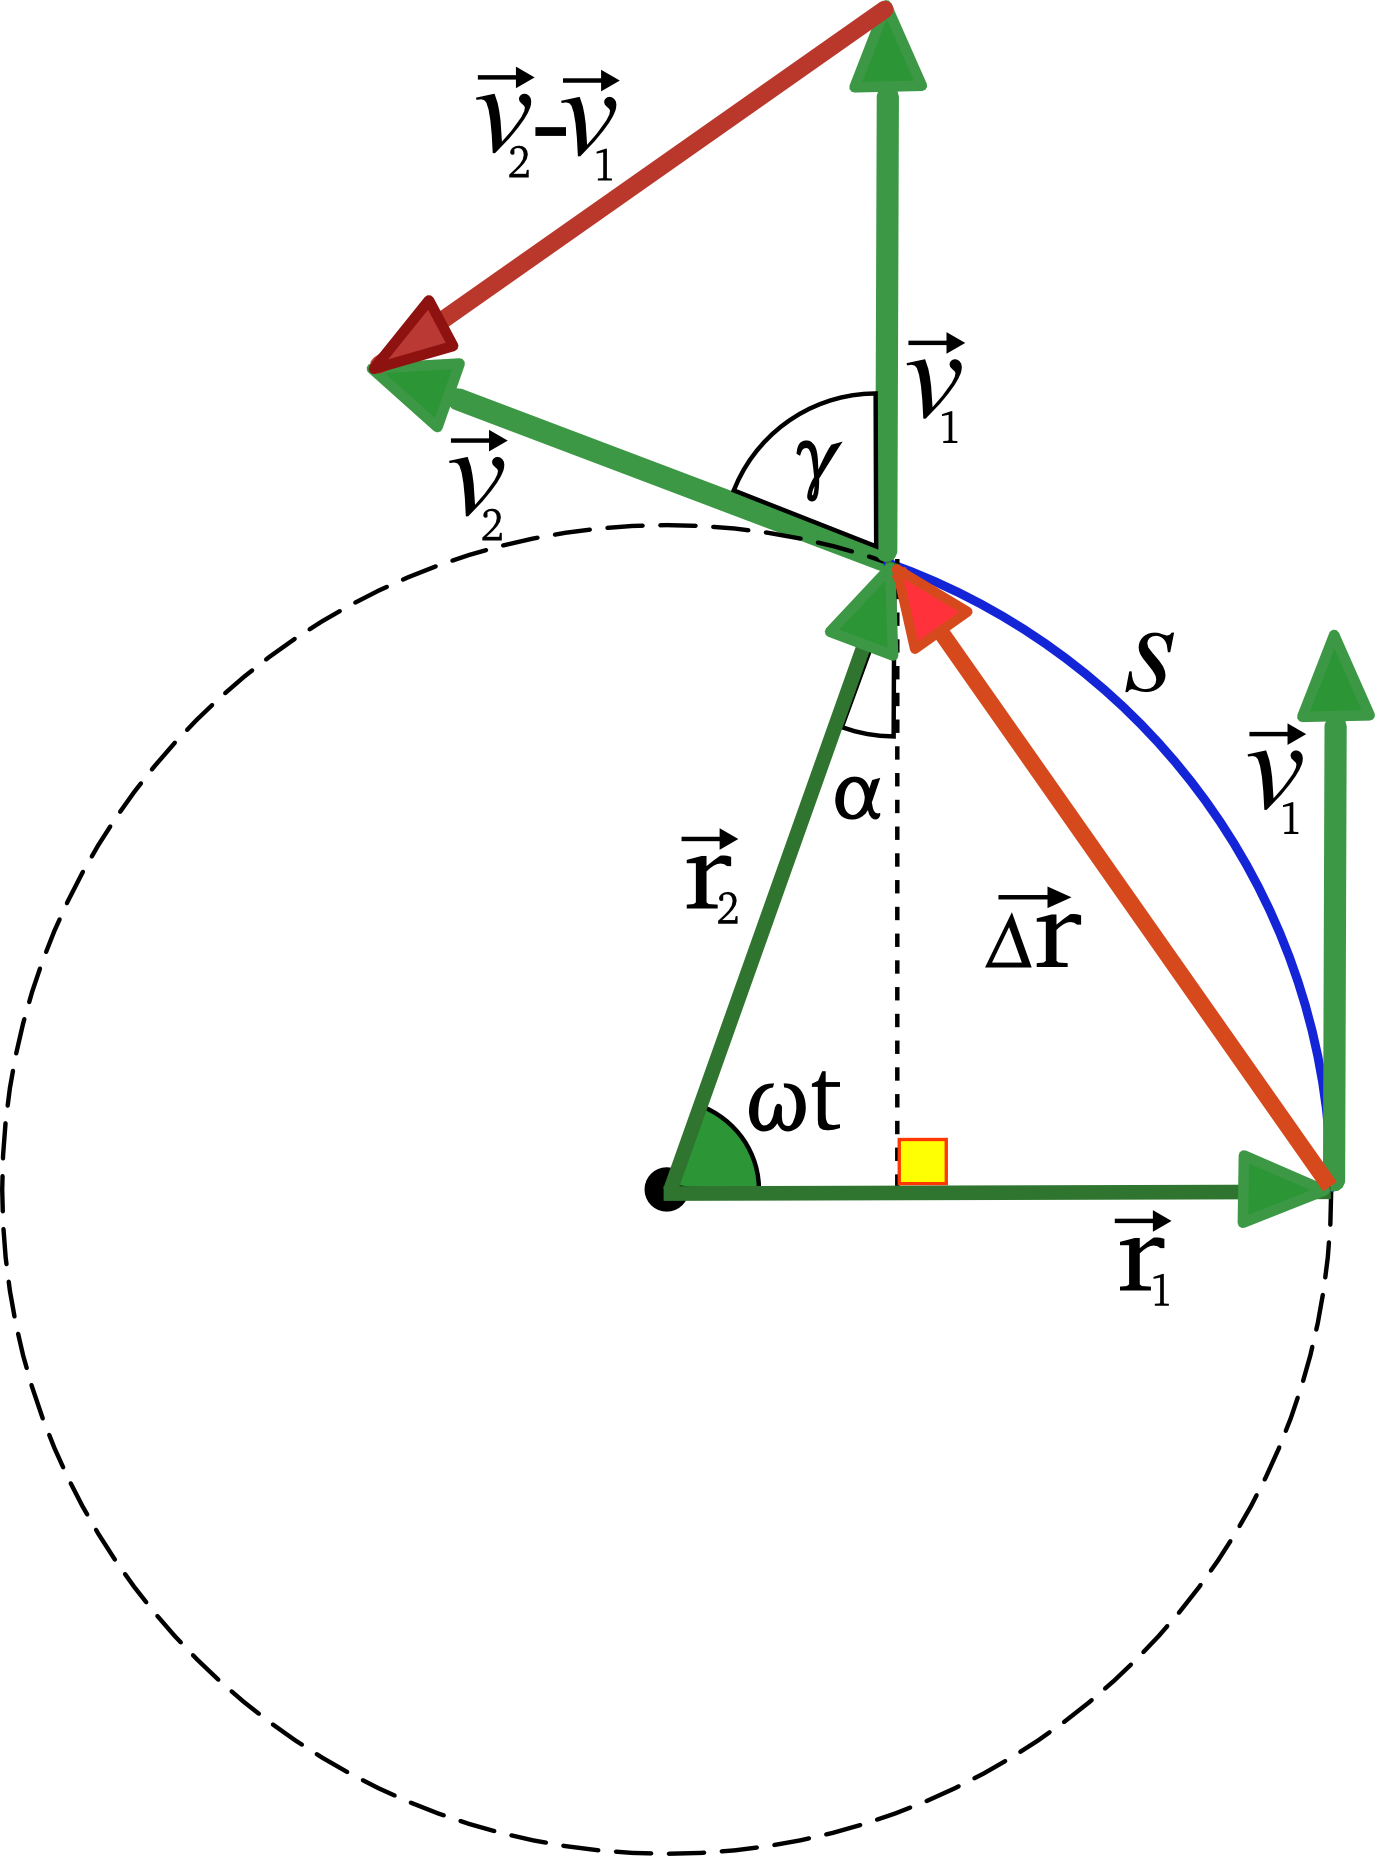
\includegraphics[width=0.4\textwidth]{./immagini/vet_acc_calc.png}
 % vet_acc_calc.png: 1375x1856 pixel, 400dpi, 8.73x11.79 cm, bb=0 0 248 334
 \caption{Calcolo del valore del modulo dell'accelerazione media}
 \label{fig:cal_acc}
\end{figure}
Notiamo subito che i due triangoli riportati in figura [\ref{fig:cal_acc}] sono isosceli dato che per uno i lati sono rappresentati da due raggi della circonferenza, mentre per l'altro da due vettori velocità che sappiamo avere lo stesso modulo, notiamo poi che l'ampiezza dell'angolo $\gamma$ è $\omega t$ questo ci assicura che i due triangoli isosceli, di cui sopra, sono simili e per tanto i rapporti tra lati omologhi dei due triangoli saranno uguali. Questa considerazione ci permette di scrivere:
\begin{equation}\label{eq:rapp_v}
 \frac{\Delta r}{r}=\frac{\Delta v}{ v}
\end{equation}
dove si sono usati i moduli dei vettori posizione e velocità e rispettive variazioni.
La relazione [\ref{eq:rapp_v}] ci permette così di calcolare il modulo della variazione di velocità:
\begin{equation}
 \Delta v=\frac{\Delta r}{r}v
\end{equation}
utilizzando ora la definizione di accelerazione media otteniamo:
\begin{equation}\label{eq:acc_media_for}
 a_m=\frac{\Delta v}{\Delta t}=\frac{\Delta r}{\Delta t}\frac{v}{r}
\end{equation}
analizziamo il fattore $\Delta r/\Delta t$, possiamo notare che quando $\Delta t$ tende a diventare sempre più piccolo l'arco $S$ sotteso dalla corda $\Delta\mathbf{r}$ e la corda stessa diventano indistinguibili quindi dalla definizione di velocità nel moto lineare uniforme posso dire che per $\Delta t$ ``piccolo'' $\Delta r/\Delta t\simeq v$. Questa constatazione ci permette di ricavare il modulo dell'accelerazione istantanea dalla [\ref{eq:acc_media_for}]:
\begin{equation}
 a=v\frac{v}{r}=\frac{v^2}{r}=\omega^2r
\end{equation}
Detto tutto ciò possiamo finalmente scrivere il vettore accelerazione istantanea:
\begin{equation}
 \mathbf{a}=\left(-\frac{v^2}{r}\cos (\omega t),-\frac{v^2}{r}\sin (\omega t)\right)=(-\omega^2r\cos(\omega t),-\omega^2r\sin (\omega t))
\end{equation}



\end{document}